\documentclass[]{beamer}

\usepackage{tikz}
\usetikzlibrary{shapes.geometric, arrows}
\tikzstyle{result} = [rectangle, rounded corners, minimum width=3cm, minimum height=0.5cm, text centered, draw=black, fill=green!30]
\tikzstyle{process} = [rectangle, minimum width=3cm, minimum height=0.5cm, text centered, draw=black, fill=orange!30]
\tikzstyle{arrow}= [thick,->,>=stealth]
\usepackage{movie15}
\usepackage{lipsum}
\usepackage{pgfpages}
\usepackage{graphicx}
\usepackage[dutch]{babel}
\graphicspath{{img/}}

\mode<handout>{%
%	\setbeameroption{show notes}
}

\usetheme{AnnArbor}
\usecolortheme{beaver}
\usepackage{graphicx}

\graphicspath{{./img/}}


\begin{document}	
	\begin{frame}{Vorige week}
		\begin{itemize}
			\item View Invariantie (hoe rotatie uitvoeren)
			\item Schaal (welke joint als norm gebruiken)
			\item (Code profiling)
		\end{itemize}
	\end{frame}
	\begin{frame}{Preprocessing}
			\begin{figure}
				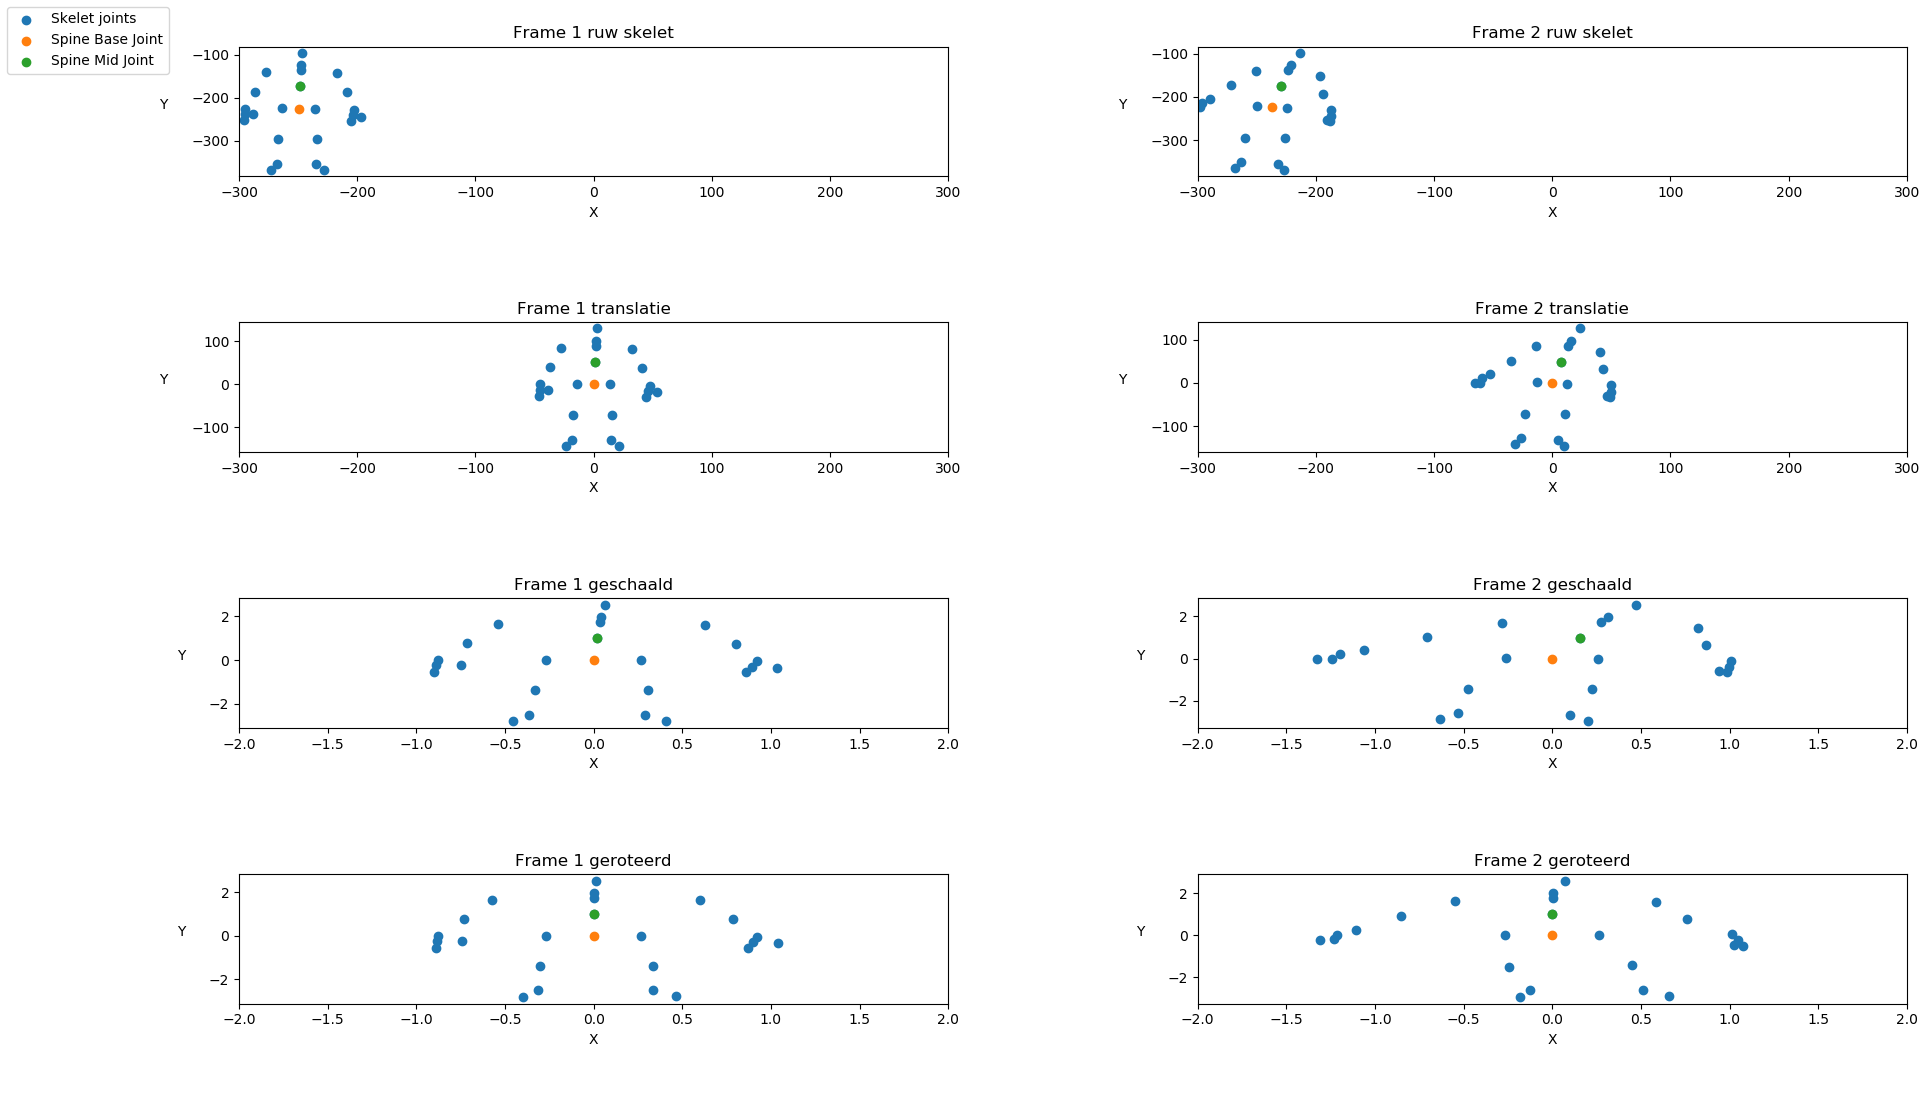
\includegraphics[width=\textwidth]{skeleton_preprocessing}
			\end{figure}
	\end{frame}
	\begin{frame}{Classification}
		\begin{figure}
			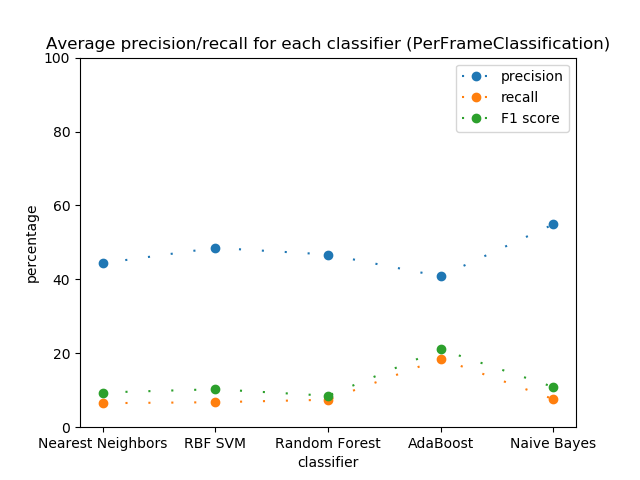
\includegraphics[width=0.7\textwidth]{PerFrameClassification}
		\end{figure} 
	\end{frame}
	\begin{frame}{Classification}
		\begin{figure}
			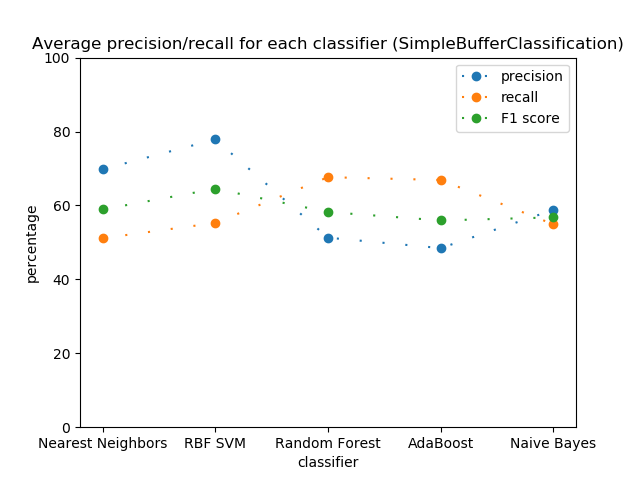
\includegraphics[width=0.7\textwidth]{SimpleBufferClassification}
		\end{figure} 
	\end{frame}
	\begin{frame}{Classification}
		\begin{figure}
			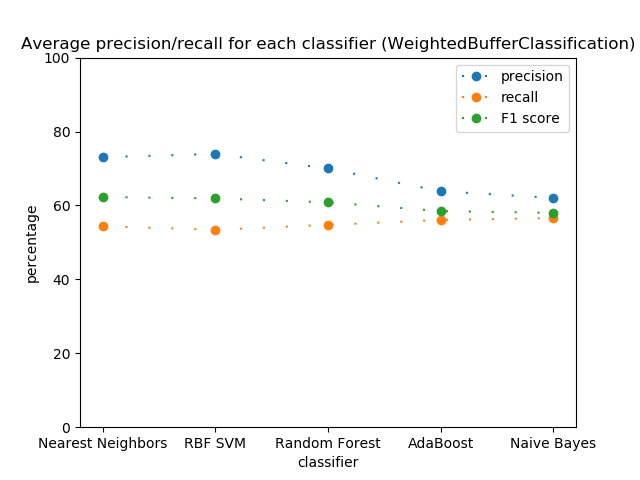
\includegraphics[width=0.7\textwidth]{WeightedBufferClassification}
		\end{figure} 
	\end{frame}
\end{document}